\documentclass{article}\usepackage[]{graphicx}\usepackage[]{color}
%% maxwidth is the original width if it is less than linewidth
%% otherwise use linewidth (to make sure the graphics do not exceed the margin)
\makeatletter
\def\maxwidth{ %
  \ifdim\Gin@nat@width>\linewidth
    \linewidth
  \else
    \Gin@nat@width
  \fi
}
\makeatother

\definecolor{fgcolor}{rgb}{0.345, 0.345, 0.345}
\newcommand{\hlnum}[1]{\textcolor[rgb]{0.686,0.059,0.569}{#1}}%
\newcommand{\hlstr}[1]{\textcolor[rgb]{0.192,0.494,0.8}{#1}}%
\newcommand{\hlcom}[1]{\textcolor[rgb]{0.678,0.584,0.686}{\textit{#1}}}%
\newcommand{\hlopt}[1]{\textcolor[rgb]{0,0,0}{#1}}%
\newcommand{\hlstd}[1]{\textcolor[rgb]{0.345,0.345,0.345}{#1}}%
\newcommand{\hlkwa}[1]{\textcolor[rgb]{0.161,0.373,0.58}{\textbf{#1}}}%
\newcommand{\hlkwb}[1]{\textcolor[rgb]{0.69,0.353,0.396}{#1}}%
\newcommand{\hlkwc}[1]{\textcolor[rgb]{0.333,0.667,0.333}{#1}}%
\newcommand{\hlkwd}[1]{\textcolor[rgb]{0.737,0.353,0.396}{\textbf{#1}}}%

\usepackage{framed}
\makeatletter
\newenvironment{kframe}{%
 \def\at@end@of@kframe{}%
 \ifinner\ifhmode%
  \def\at@end@of@kframe{\end{minipage}}%
  \begin{minipage}{\columnwidth}%
 \fi\fi%
 \def\FrameCommand##1{\hskip\@totalleftmargin \hskip-\fboxsep
 \colorbox{shadecolor}{##1}\hskip-\fboxsep
     % There is no \\@totalrightmargin, so:
     \hskip-\linewidth \hskip-\@totalleftmargin \hskip\columnwidth}%
 \MakeFramed {\advance\hsize-\width
   \@totalleftmargin\z@ \linewidth\hsize
   \@setminipage}}%
 {\par\unskip\endMakeFramed%
 \at@end@of@kframe}
\makeatother

\definecolor{shadecolor}{rgb}{.97, .97, .97}
\definecolor{messagecolor}{rgb}{0, 0, 0}
\definecolor{warningcolor}{rgb}{1, 0, 1}
\definecolor{errorcolor}{rgb}{1, 0, 0}
\newenvironment{knitrout}{}{} % an empty environment to be redefined in TeX

\usepackage{alltt}
\usepackage[vmargin=1in,hmargin=1in]{geometry}
\usepackage{enumerate}
\IfFileExists{upquote.sty}{\usepackage{upquote}}{}
\begin{document}
\title{Homework 1}
\date{BSAD 8700 - Business Analytics\\ Due: January 19, 2015}
\author{Cally Thompson, Diane Keeton, Evan Porter, Jace Crist, Kayla Uhing\\ University of Nebraska at Omaha}
\maketitle

\textbf{ANSWER FOR 8:} \\


\begin{enumerate}[(a)]
\item
\begin{knitrout}
\definecolor{shadecolor}{rgb}{0.969, 0.969, 0.969}\color{fgcolor}\begin{kframe}
\begin{alltt}
\hlstd{college}\hlkwb{<-}\hlkwd{read.csv}\hlstd{(}\hlstr{"college.csv"}\hlstd{)}
\hlkwd{tail}\hlstd{(college)}
\end{alltt}
\begin{verbatim}
##                                   X Private  Apps Accept Enroll Top10perc
## 772 Worcester Polytechnic Institute     Yes  2768   2314    682        49
## 773         Worcester State College      No  2197   1515    543         4
## 774               Xavier University     Yes  1959   1805    695        24
## 775  Xavier University of Louisiana     Yes  2097   1915    695        34
## 776                 Yale University     Yes 10705   2453   1317        95
## 777    York College of Pennsylvania     Yes  2989   1855    691        28
##     Top25perc F.Undergrad P.Undergrad Outstate Room.Board Books Personal
## 772        86        2802          86    15884       5370   530      730
## 773        26        3089        2029     6797       3900   500     1200
## 774        47        2849        1107    11520       4960   600     1250
## 775        61        2793         166     6900       4200   617      781
## 776        99        5217          83    19840       6510   630     2115
## 777        63        2988        1726     4990       3560   500     1250
##     PhD Terminal S.F.Ratio perc.alumni Expend Grad.Rate
## 772  92       94      15.2          34  10774        82
## 773  60       60      21.0          14   4469        40
## 774  73       75      13.3          31   9189        83
## 775  67       75      14.4          20   8323        49
## 776  96       96       5.8          49  40386        99
## 777  75       75      18.1          28   4509        99
\end{verbatim}
\end{kframe}
\end{knitrout}
\item
\begin{knitrout}
\definecolor{shadecolor}{rgb}{0.969, 0.969, 0.969}\color{fgcolor}\begin{kframe}
\begin{alltt}
\hlcom{#fix(college)}
\hlkwd{rownames}\hlstd{(college)}\hlkwb{=}\hlstd{college[,}\hlnum{1}\hlstd{]}
\hlcom{#fix(college)}
\hlstd{college}\hlkwb{=}\hlstd{college[,}\hlopt{-}\hlnum{1}\hlstd{]}
\hlcom{#fix(college)}
\end{alltt}
\end{kframe}
\end{knitrout}
Fix 1$:$ \\
\begin{knitrout}
\definecolor{shadecolor}{rgb}{0.969, 0.969, 0.969}\color{fgcolor}\begin{kframe}
\begin{alltt}
\hlstd{a}\hlkwb{<-}\hlkwd{readPNG}\hlstd{(}\hlstr{"PNG1.png"}\hlstd{)}
\hlstd{aRaster} \hlkwb{<-} \hlkwd{as.raster}\hlstd{(a)}
\hlkwd{grid.raster}\hlstd{(aRaster)}
\end{alltt}
\end{kframe}
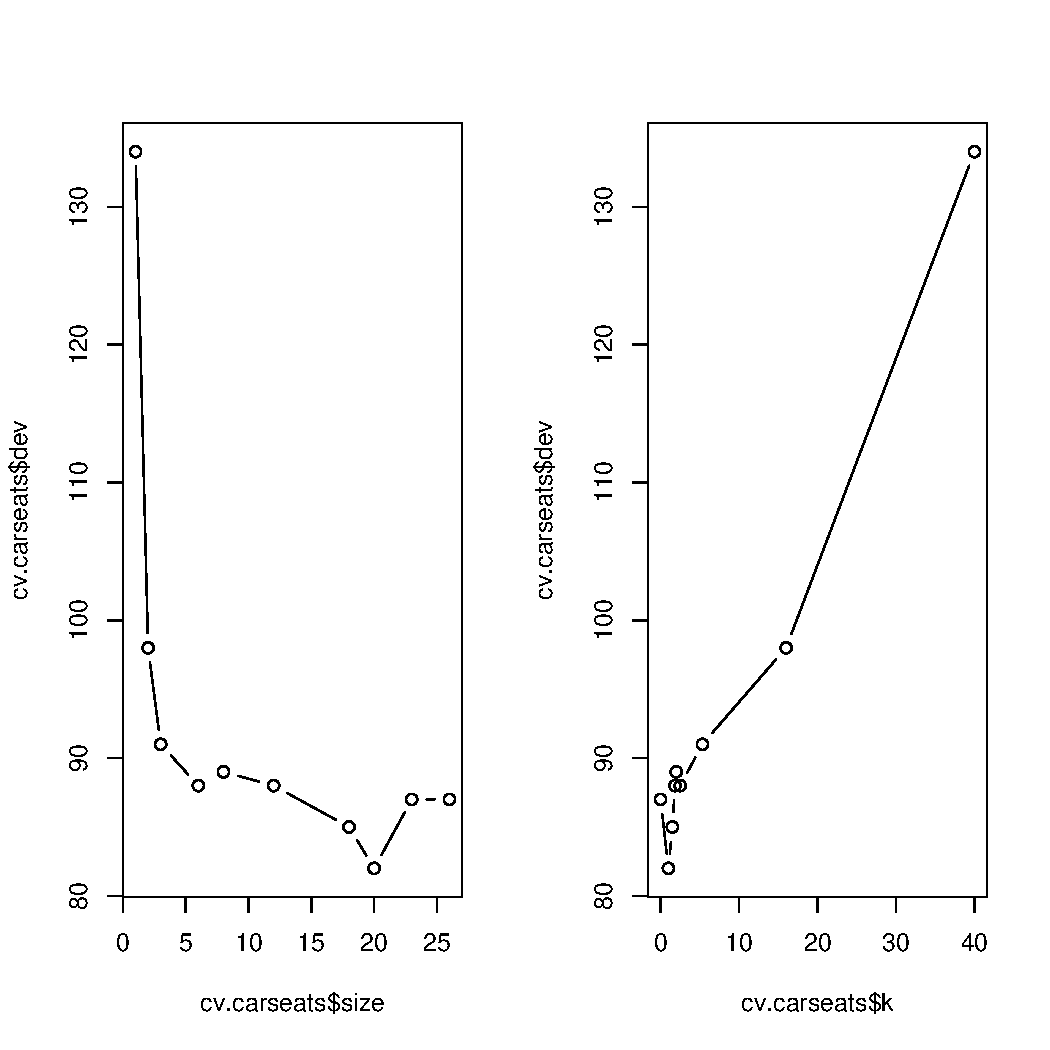
\includegraphics[width=\maxwidth]{figure/unnamed-chunk-4-1} 

\end{knitrout}
Fix 2$:$ \\
\begin{knitrout}
\definecolor{shadecolor}{rgb}{0.969, 0.969, 0.969}\color{fgcolor}\begin{kframe}
\begin{alltt}
\hlstd{b}\hlkwb{<-}\hlkwd{readPNG}\hlstd{(}\hlstr{"PNG2.png"}\hlstd{)}
\hlstd{bRaster} \hlkwb{<-} \hlkwd{as.raster}\hlstd{(b)}
\hlkwd{grid.raster}\hlstd{(bRaster)}
\end{alltt}
\end{kframe}
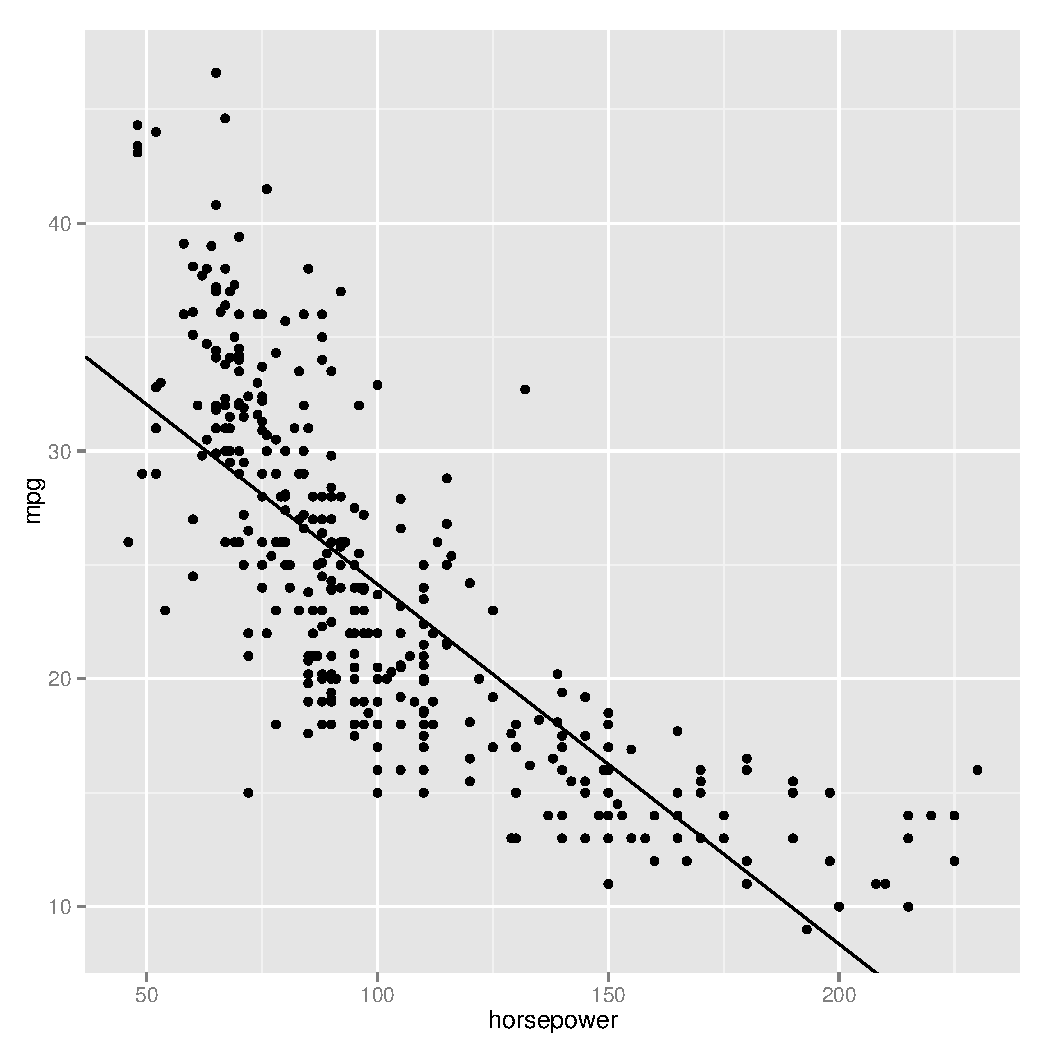
\includegraphics[width=\maxwidth]{figure/unnamed-chunk-5-1} 

\end{knitrout}
Fix 3$:$ \\
\begin{knitrout}
\definecolor{shadecolor}{rgb}{0.969, 0.969, 0.969}\color{fgcolor}\begin{kframe}
\begin{alltt}
\hlstd{c}\hlkwb{<-}\hlkwd{readPNG}\hlstd{(}\hlstr{"PNG3.png"}\hlstd{)}
\hlstd{cRaster} \hlkwb{<-} \hlkwd{as.raster}\hlstd{(c)}
\hlkwd{grid.raster}\hlstd{(cRaster)}
\end{alltt}
\end{kframe}
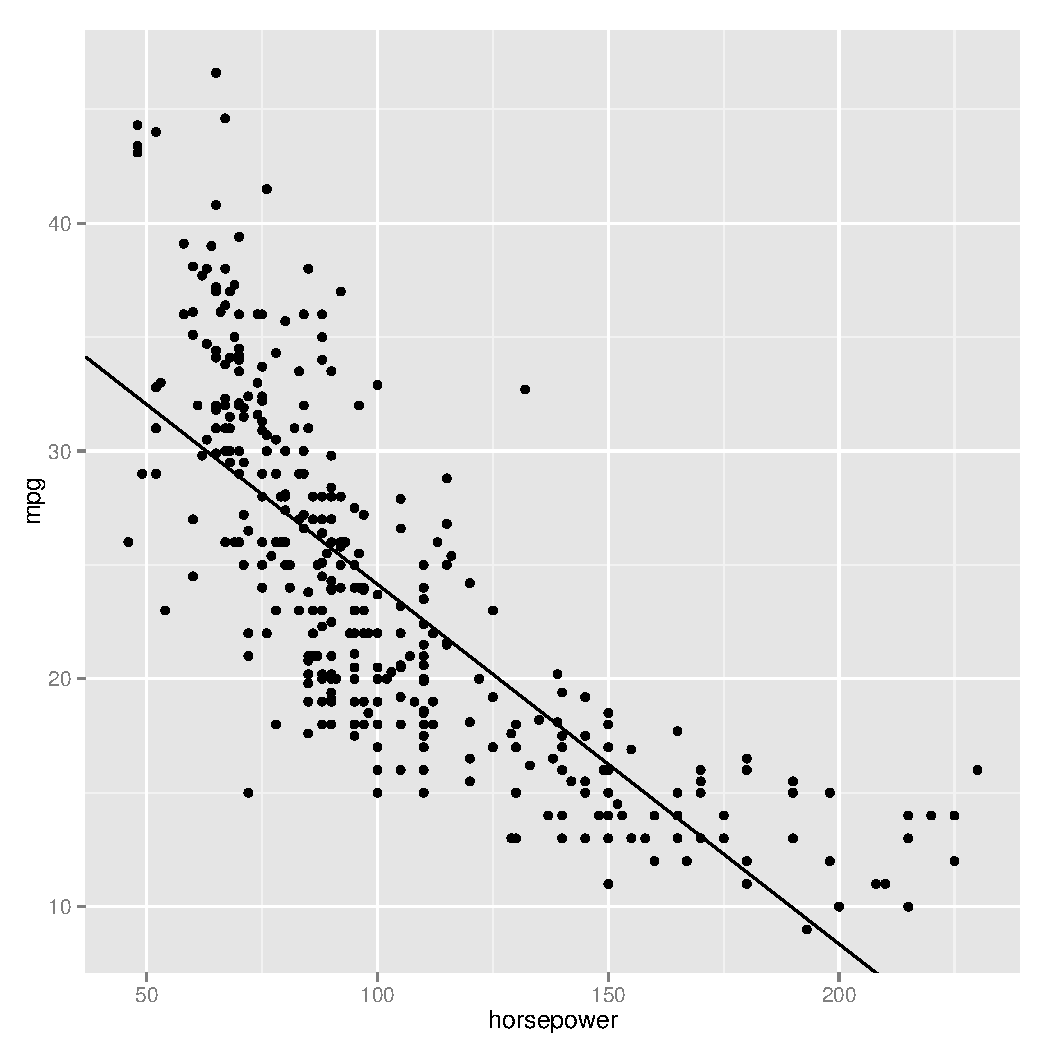
\includegraphics[width=\maxwidth]{figure/unnamed-chunk-6-1} 

\end{knitrout}

\item
\begin{enumerate}[(i)]
\item
\begin{knitrout}
\definecolor{shadecolor}{rgb}{0.969, 0.969, 0.969}\color{fgcolor}\begin{kframe}
\begin{alltt}
\hlkwd{summary}\hlstd{(college)}
\end{alltt}
\begin{verbatim}
##  Private        Apps           Accept          Enroll       Top10perc    
##  No :212   Min.   :   81   Min.   :   72   Min.   :  35   Min.   : 1.00  
##  Yes:565   1st Qu.:  776   1st Qu.:  604   1st Qu.: 242   1st Qu.:15.00  
##            Median : 1558   Median : 1110   Median : 434   Median :23.00  
##            Mean   : 3002   Mean   : 2019   Mean   : 780   Mean   :27.56  
##            3rd Qu.: 3624   3rd Qu.: 2424   3rd Qu.: 902   3rd Qu.:35.00  
##            Max.   :48094   Max.   :26330   Max.   :6392   Max.   :96.00  
##    Top25perc      F.Undergrad     P.Undergrad         Outstate    
##  Min.   :  9.0   Min.   :  139   Min.   :    1.0   Min.   : 2340  
##  1st Qu.: 41.0   1st Qu.:  992   1st Qu.:   95.0   1st Qu.: 7320  
##  Median : 54.0   Median : 1707   Median :  353.0   Median : 9990  
##  Mean   : 55.8   Mean   : 3700   Mean   :  855.3   Mean   :10441  
##  3rd Qu.: 69.0   3rd Qu.: 4005   3rd Qu.:  967.0   3rd Qu.:12925  
##  Max.   :100.0   Max.   :31643   Max.   :21836.0   Max.   :21700  
##    Room.Board       Books           Personal         PhD        
##  Min.   :1780   Min.   :  96.0   Min.   : 250   Min.   :  8.00  
##  1st Qu.:3597   1st Qu.: 470.0   1st Qu.: 850   1st Qu.: 62.00  
##  Median :4200   Median : 500.0   Median :1200   Median : 75.00  
##  Mean   :4358   Mean   : 549.4   Mean   :1341   Mean   : 72.66  
##  3rd Qu.:5050   3rd Qu.: 600.0   3rd Qu.:1700   3rd Qu.: 85.00  
##  Max.   :8124   Max.   :2340.0   Max.   :6800   Max.   :103.00  
##     Terminal       S.F.Ratio      perc.alumni        Expend     
##  Min.   : 24.0   Min.   : 2.50   Min.   : 0.00   Min.   : 3186  
##  1st Qu.: 71.0   1st Qu.:11.50   1st Qu.:13.00   1st Qu.: 6751  
##  Median : 82.0   Median :13.60   Median :21.00   Median : 8377  
##  Mean   : 79.7   Mean   :14.09   Mean   :22.74   Mean   : 9660  
##  3rd Qu.: 92.0   3rd Qu.:16.50   3rd Qu.:31.00   3rd Qu.:10830  
##  Max.   :100.0   Max.   :39.80   Max.   :64.00   Max.   :56233  
##    Grad.Rate     
##  Min.   : 10.00  
##  1st Qu.: 53.00  
##  Median : 65.00  
##  Mean   : 65.46  
##  3rd Qu.: 78.00  
##  Max.   :118.00
\end{verbatim}
\end{kframe}
\end{knitrout}
\item
\begin{knitrout}
\definecolor{shadecolor}{rgb}{0.969, 0.969, 0.969}\color{fgcolor}\begin{kframe}
\begin{alltt}
\hlkwd{pairs}\hlstd{(college[,}\hlnum{1}\hlopt{:}\hlnum{10}\hlstd{])}
\end{alltt}
\end{kframe}
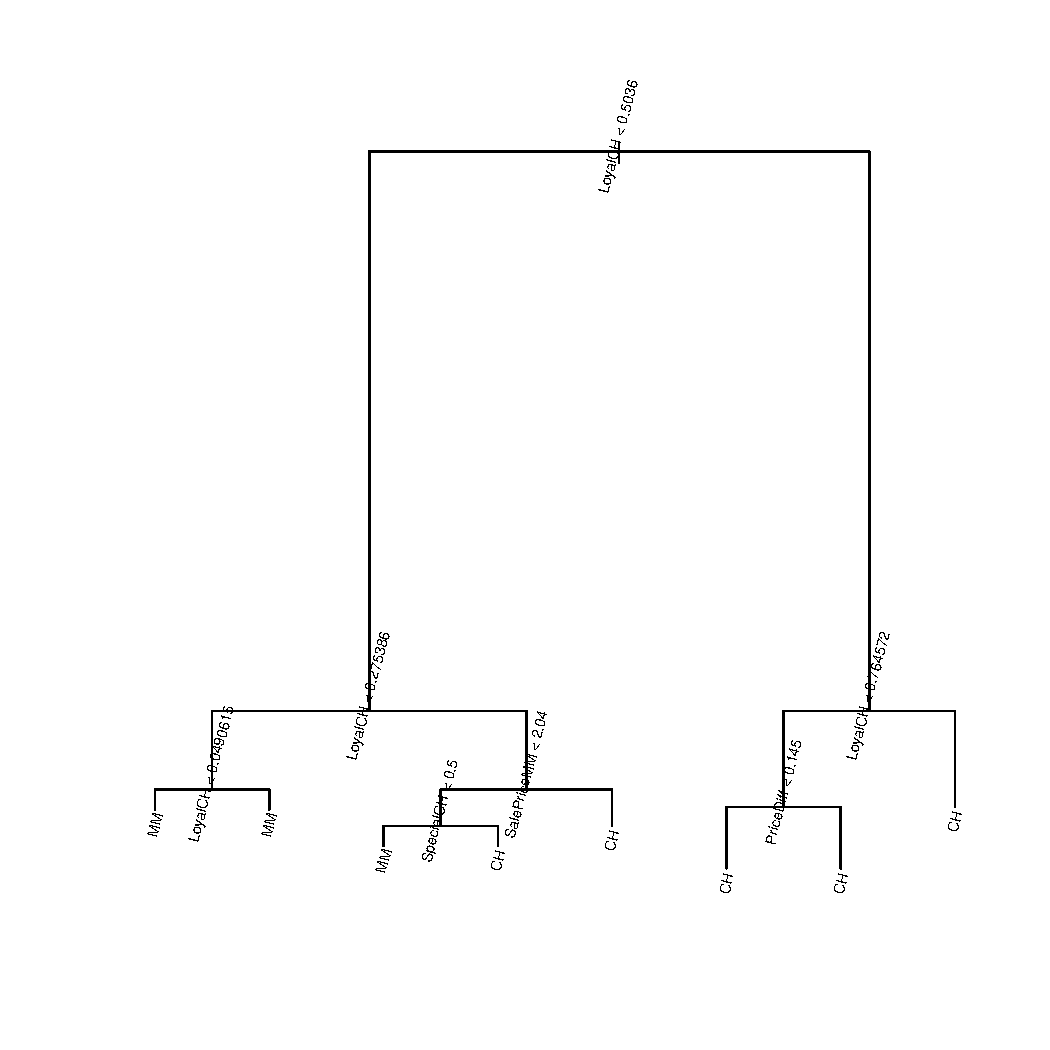
\includegraphics[width=\maxwidth]{figure/unnamed-chunk-8-1} 

\end{knitrout}
\item
\begin{knitrout}
\definecolor{shadecolor}{rgb}{0.969, 0.969, 0.969}\color{fgcolor}\begin{kframe}
\begin{alltt}
\hlkwd{attach}\hlstd{(college)}
\hlkwd{plot}\hlstd{(Outstate}\hlopt{~}\hlstd{Private)}
\end{alltt}
\end{kframe}
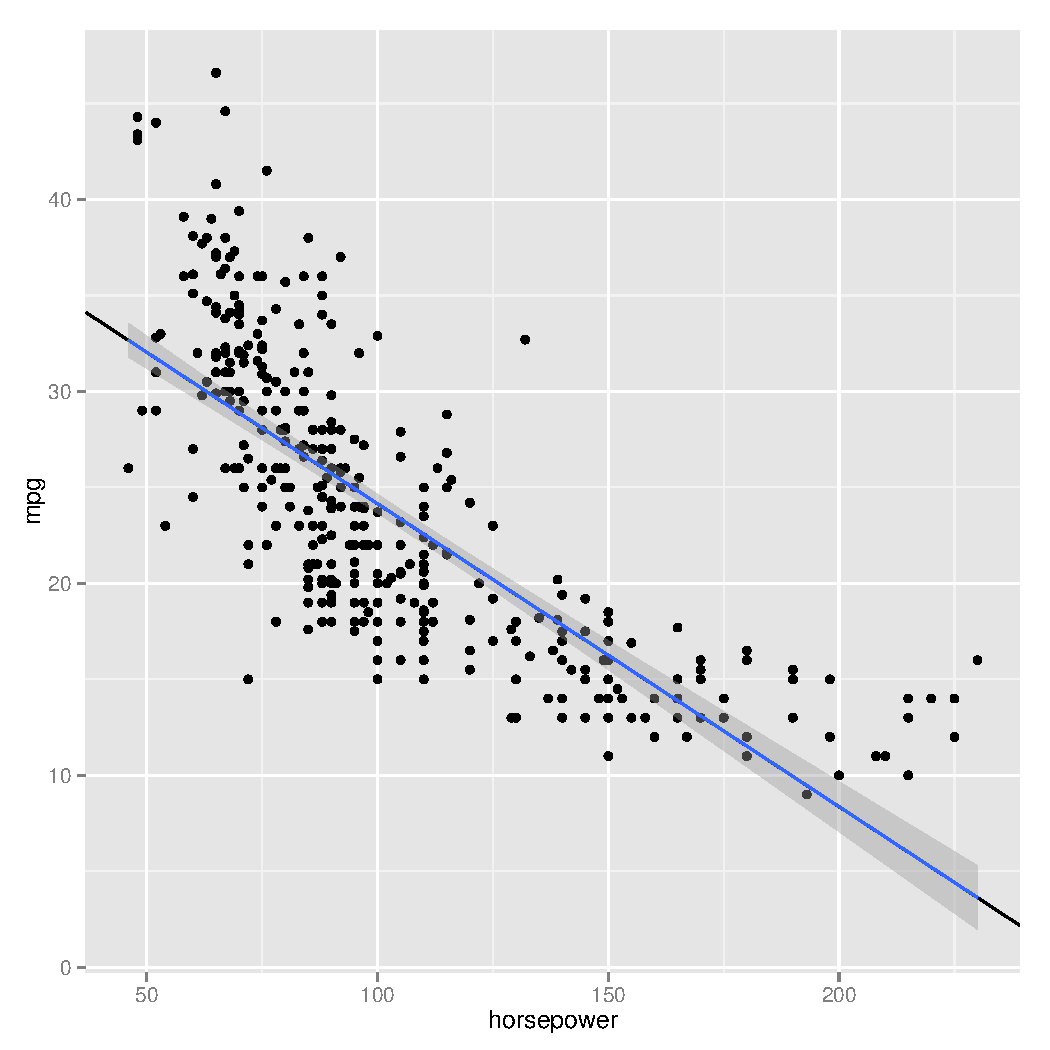
\includegraphics[width=\maxwidth]{figure/unnamed-chunk-9-1} 

\end{knitrout}
\item
There are 78 elite Universities.
\begin{knitrout}
\definecolor{shadecolor}{rgb}{0.969, 0.969, 0.969}\color{fgcolor}\begin{kframe}
\begin{alltt}
\hlstd{Elite}\hlkwb{=}\hlkwd{rep}\hlstd{(}\hlstr{"No"}\hlstd{,}\hlkwd{nrow}\hlstd{(college))}
\hlstd{Elite[college}\hlopt{$}\hlstd{Top10perc}\hlopt{>}\hlnum{50}\hlstd{]}\hlkwb{=}\hlstr{"Yes"}
\hlstd{Elite}\hlkwb{=}\hlkwd{as.factor}\hlstd{(Elite)}
\hlstd{college}\hlkwb{=}\hlkwd{data.frame}\hlstd{(college ,Elite)}
\hlkwd{summary}\hlstd{(college)}
\end{alltt}
\begin{verbatim}
##  Private        Apps           Accept          Enroll       Top10perc    
##  No :212   Min.   :   81   Min.   :   72   Min.   :  35   Min.   : 1.00  
##  Yes:565   1st Qu.:  776   1st Qu.:  604   1st Qu.: 242   1st Qu.:15.00  
##            Median : 1558   Median : 1110   Median : 434   Median :23.00  
##            Mean   : 3002   Mean   : 2019   Mean   : 780   Mean   :27.56  
##            3rd Qu.: 3624   3rd Qu.: 2424   3rd Qu.: 902   3rd Qu.:35.00  
##            Max.   :48094   Max.   :26330   Max.   :6392   Max.   :96.00  
##    Top25perc      F.Undergrad     P.Undergrad         Outstate    
##  Min.   :  9.0   Min.   :  139   Min.   :    1.0   Min.   : 2340  
##  1st Qu.: 41.0   1st Qu.:  992   1st Qu.:   95.0   1st Qu.: 7320  
##  Median : 54.0   Median : 1707   Median :  353.0   Median : 9990  
##  Mean   : 55.8   Mean   : 3700   Mean   :  855.3   Mean   :10441  
##  3rd Qu.: 69.0   3rd Qu.: 4005   3rd Qu.:  967.0   3rd Qu.:12925  
##  Max.   :100.0   Max.   :31643   Max.   :21836.0   Max.   :21700  
##    Room.Board       Books           Personal         PhD        
##  Min.   :1780   Min.   :  96.0   Min.   : 250   Min.   :  8.00  
##  1st Qu.:3597   1st Qu.: 470.0   1st Qu.: 850   1st Qu.: 62.00  
##  Median :4200   Median : 500.0   Median :1200   Median : 75.00  
##  Mean   :4358   Mean   : 549.4   Mean   :1341   Mean   : 72.66  
##  3rd Qu.:5050   3rd Qu.: 600.0   3rd Qu.:1700   3rd Qu.: 85.00  
##  Max.   :8124   Max.   :2340.0   Max.   :6800   Max.   :103.00  
##     Terminal       S.F.Ratio      perc.alumni        Expend     
##  Min.   : 24.0   Min.   : 2.50   Min.   : 0.00   Min.   : 3186  
##  1st Qu.: 71.0   1st Qu.:11.50   1st Qu.:13.00   1st Qu.: 6751  
##  Median : 82.0   Median :13.60   Median :21.00   Median : 8377  
##  Mean   : 79.7   Mean   :14.09   Mean   :22.74   Mean   : 9660  
##  3rd Qu.: 92.0   3rd Qu.:16.50   3rd Qu.:31.00   3rd Qu.:10830  
##  Max.   :100.0   Max.   :39.80   Max.   :64.00   Max.   :56233  
##    Grad.Rate      Elite    
##  Min.   : 10.00   No :699  
##  1st Qu.: 53.00   Yes: 78  
##  Median : 65.00            
##  Mean   : 65.46            
##  3rd Qu.: 78.00            
##  Max.   :118.00
\end{verbatim}
\begin{alltt}
\hlkwd{plot}\hlstd{(college}\hlopt{$}\hlstd{Outstate}\hlopt{~}\hlstd{college}\hlopt{$}\hlstd{Elite)}
\end{alltt}
\end{kframe}
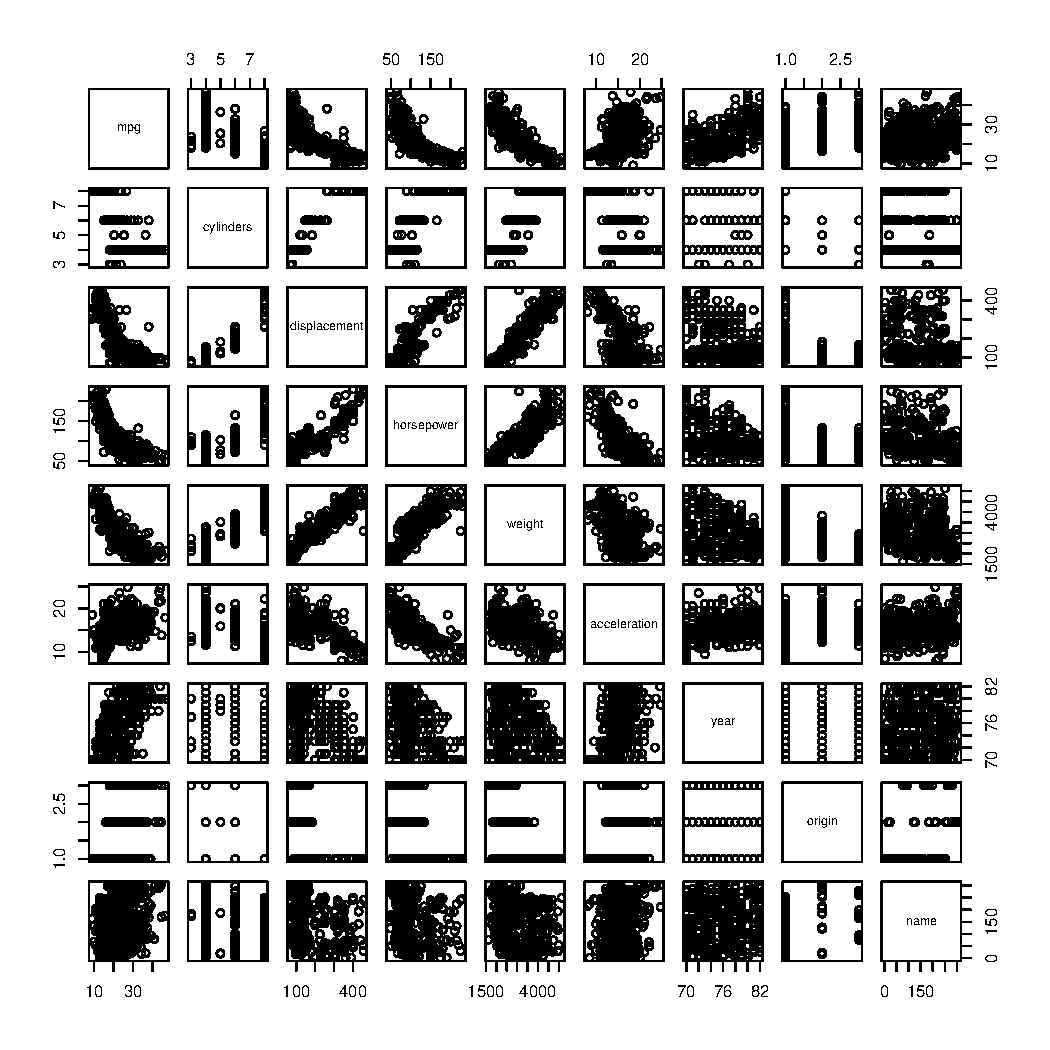
\includegraphics[width=\maxwidth]{figure/unnamed-chunk-10-1} 

\end{knitrout}

\item
\begin{knitrout}
\definecolor{shadecolor}{rgb}{0.969, 0.969, 0.969}\color{fgcolor}\begin{kframe}
\begin{alltt}
\hlkwd{hist}\hlstd{(Apps)}
\hlkwd{par}\hlstd{(}\hlkwc{mfrow}\hlstd{=}\hlkwd{c}\hlstd{(}\hlnum{2}\hlstd{,}\hlnum{2}\hlstd{))}
\hlkwd{hist}\hlstd{(Apps)}
\hlkwd{hist}\hlstd{(Accept)}
\hlkwd{hist}\hlstd{(Books)}
\hlkwd{hist}\hlstd{(PhD)}
\end{alltt}
\end{kframe}
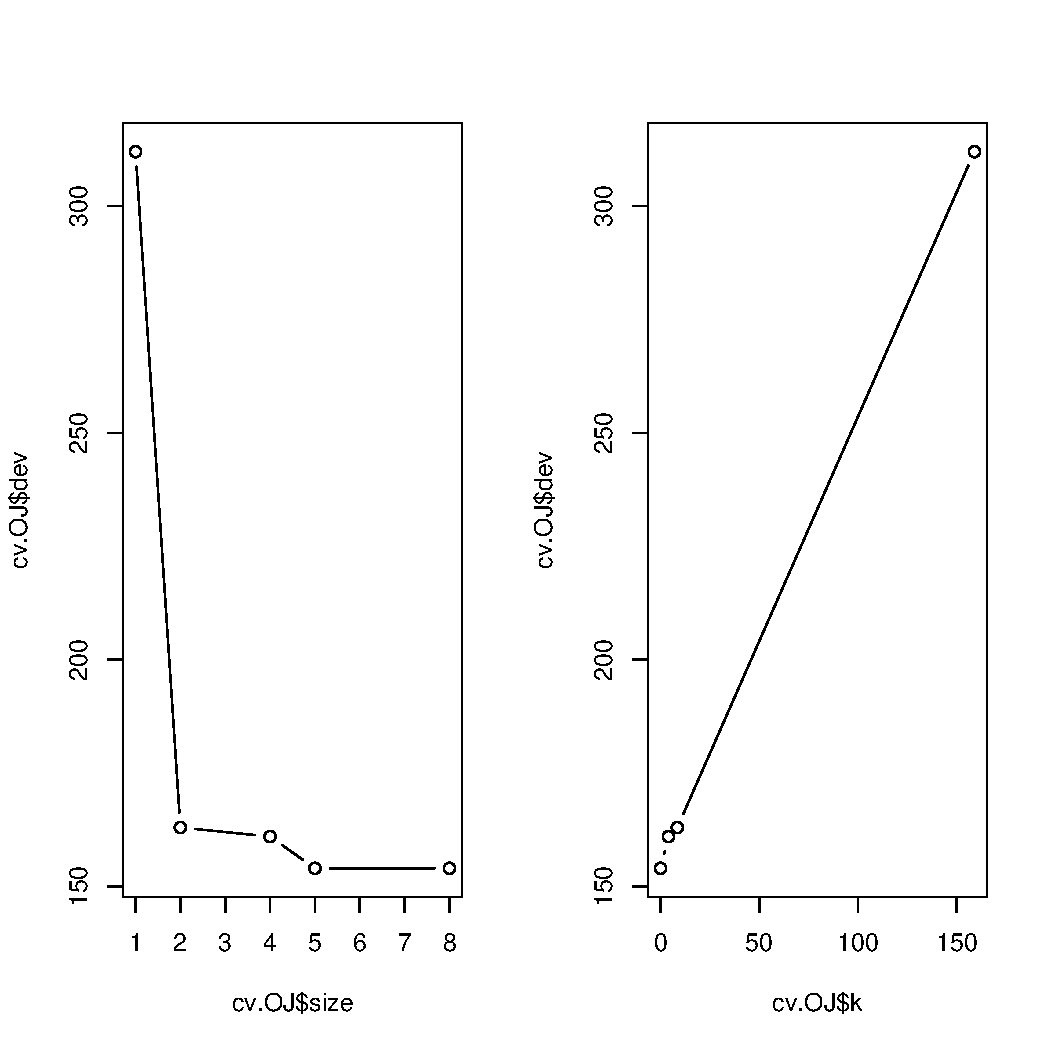
\includegraphics[width=\maxwidth]{figure/unnamed-chunk-11-1} 

\end{knitrout}
\item
After reviewing the data and performing the basic functions of R, we have found that there are numerous ways to extract information. There are also multiple different ways to find this data, there are no "right" or "wrong" ways of doing so. Through analyzing qualitative variables, R allows you to get the data you will need, although proper coding must be enforced. The basic commands were a bit difficult to figure out, but the more we did the assignment, the more we started learning what we were actually doing. The visuals of the Histograms and Plot graphs were helpful in dissecting the data. \\
\end{enumerate}
\end{enumerate}


\textbf{ANSWER FOR 10:}

\begin{enumerate}[(a)]
\item
\begin{knitrout}
\definecolor{shadecolor}{rgb}{0.969, 0.969, 0.969}\color{fgcolor}\begin{kframe}
\begin{alltt}
\hlkwd{tail}\hlstd{(Boston)}
\end{alltt}
\begin{verbatim}
##        crim zn indus chas   nox    rm  age    dis rad tax ptratio  black
## 501 0.22438  0  9.69    0 0.585 6.027 79.7 2.4982   6 391    19.2 396.90
## 502 0.06263  0 11.93    0 0.573 6.593 69.1 2.4786   1 273    21.0 391.99
## 503 0.04527  0 11.93    0 0.573 6.120 76.7 2.2875   1 273    21.0 396.90
## 504 0.06076  0 11.93    0 0.573 6.976 91.0 2.1675   1 273    21.0 396.90
## 505 0.10959  0 11.93    0 0.573 6.794 89.3 2.3889   1 273    21.0 393.45
## 506 0.04741  0 11.93    0 0.573 6.030 80.8 2.5050   1 273    21.0 396.90
##     lstat medv
## 501 14.33 16.8
## 502  9.67 22.4
## 503  9.08 20.6
## 504  5.64 23.9
## 505  6.48 22.0
## 506  7.88 11.9
\end{verbatim}
\begin{alltt}
\hlkwd{dim}\hlstd{(Boston)}
\end{alltt}
\begin{verbatim}
## [1] 506  14
\end{verbatim}
\begin{alltt}
\hlcom{#?(Boston)}
\end{alltt}
\end{kframe}
\end{knitrout}
The Boston data frame has 506 rows and 14 columns. \\ The columns and rows represent data including crime, age and median value of owner-occupied homes in \$ 1000s \\
\item
\begin{knitrout}
\definecolor{shadecolor}{rgb}{0.969, 0.969, 0.969}\color{fgcolor}\begin{kframe}
\begin{alltt}
\hlkwd{pairs}\hlstd{(Boston)}
\end{alltt}
\end{kframe}
\includegraphics[width=\maxwidth]{figure/unnamed-chunk-13-1} 
\begin{kframe}\begin{alltt}
\hlkwd{pairs}\hlstd{(Boston[,}\hlnum{1}\hlopt{:}\hlnum{7}\hlstd{])}
\end{alltt}
\end{kframe}
\includegraphics[width=\maxwidth]{figure/unnamed-chunk-13-2} 
\begin{kframe}\begin{alltt}
\hlkwd{pairs}\hlstd{(Boston[,}\hlnum{8}\hlopt{:}\hlnum{14}\hlstd{])}
\end{alltt}
\end{kframe}
\includegraphics[width=\maxwidth]{figure/unnamed-chunk-13-3} 
\begin{kframe}\begin{alltt}
\hlkwd{round}\hlstd{(}\hlkwd{cor}\hlstd{(Boston),}\hlnum{2}\hlstd{)}
\end{alltt}
\begin{verbatim}
##          crim    zn indus  chas   nox    rm   age   dis   rad   tax
## crim     1.00 -0.20  0.41 -0.06  0.42 -0.22  0.35 -0.38  0.63  0.58
## zn      -0.20  1.00 -0.53 -0.04 -0.52  0.31 -0.57  0.66 -0.31 -0.31
## indus    0.41 -0.53  1.00  0.06  0.76 -0.39  0.64 -0.71  0.60  0.72
## chas    -0.06 -0.04  0.06  1.00  0.09  0.09  0.09 -0.10 -0.01 -0.04
## nox      0.42 -0.52  0.76  0.09  1.00 -0.30  0.73 -0.77  0.61  0.67
## rm      -0.22  0.31 -0.39  0.09 -0.30  1.00 -0.24  0.21 -0.21 -0.29
## age      0.35 -0.57  0.64  0.09  0.73 -0.24  1.00 -0.75  0.46  0.51
## dis     -0.38  0.66 -0.71 -0.10 -0.77  0.21 -0.75  1.00 -0.49 -0.53
## rad      0.63 -0.31  0.60 -0.01  0.61 -0.21  0.46 -0.49  1.00  0.91
## tax      0.58 -0.31  0.72 -0.04  0.67 -0.29  0.51 -0.53  0.91  1.00
## ptratio  0.29 -0.39  0.38 -0.12  0.19 -0.36  0.26 -0.23  0.46  0.46
## black   -0.39  0.18 -0.36  0.05 -0.38  0.13 -0.27  0.29 -0.44 -0.44
## lstat    0.46 -0.41  0.60 -0.05  0.59 -0.61  0.60 -0.50  0.49  0.54
## medv    -0.39  0.36 -0.48  0.18 -0.43  0.70 -0.38  0.25 -0.38 -0.47
##         ptratio black lstat  medv
## crim       0.29 -0.39  0.46 -0.39
## zn        -0.39  0.18 -0.41  0.36
## indus      0.38 -0.36  0.60 -0.48
## chas      -0.12  0.05 -0.05  0.18
## nox        0.19 -0.38  0.59 -0.43
## rm        -0.36  0.13 -0.61  0.70
## age        0.26 -0.27  0.60 -0.38
## dis       -0.23  0.29 -0.50  0.25
## rad        0.46 -0.44  0.49 -0.38
## tax        0.46 -0.44  0.54 -0.47
## ptratio    1.00 -0.18  0.37 -0.51
## black     -0.18  1.00 -0.37  0.33
## lstat      0.37 -0.37  1.00 -0.74
## medv      -0.51  0.33 -0.74  1.00
\end{verbatim}
\end{kframe}
\end{knitrout}
There is a negative correlation between the lower status of the population (lstat) and median value of owner occupied homes (medv). This correlation could be attributed to the fact that the lower the individual status, the lower the income of the home. Another example of negative correlation would be from the nitrogen oxcide concentration (nox) and the weighted mean of distances to Boston employment centers (dis). This correlation is related to the fact that as employment centers are more spread out, the polution decreases. An example of positive correlation would be the relationship between the average number of rooms per dwelling (rm) and median value of owner occupied home (medv). This graph shows that the number of rooms in a dwelling go up as the median value of the home increases. \\

\item
\begin{knitrout}
\definecolor{shadecolor}{rgb}{0.969, 0.969, 0.969}\color{fgcolor}\begin{kframe}
\begin{alltt}
\hlkwd{ggplot}\hlstd{(Boston,} \hlkwd{aes}\hlstd{(medv,crim))}\hlopt{+}\hlkwd{geom_point}\hlstd{()}
\end{alltt}
\end{kframe}
\includegraphics[width=\maxwidth]{figure/unnamed-chunk-14-1} 

\end{knitrout}
In regard to predictors associated with crime rate, it is shown that there seems to be a relationship such that the higher the median value of the home, the lower the crime rate. \\
  
\item
\begin{knitrout}
\definecolor{shadecolor}{rgb}{0.969, 0.969, 0.969}\color{fgcolor}\begin{kframe}
\begin{alltt}
\hlkwd{write.csv}\hlstd{(Boston,} \hlstr{"Boston.csv"}\hlstd{)}
\hlcom{# colnames(Boston)}
\hlkwd{ggplot}\hlstd{(Boston,} \hlkwd{aes}\hlstd{(black,crim))}\hlopt{+}\hlkwd{geom_point}\hlstd{()}
\end{alltt}
\end{kframe}
\includegraphics[width=\maxwidth]{figure/unnamed-chunk-15-1} 
\begin{kframe}\begin{alltt}
\hlkwd{ggplot}\hlstd{(Boston,} \hlkwd{aes}\hlstd{(age,crim))}\hlopt{+}\hlkwd{geom_point}\hlstd{()}
\end{alltt}
\end{kframe}
\includegraphics[width=\maxwidth]{figure/unnamed-chunk-15-2} 
\begin{kframe}\begin{alltt}
\hlkwd{ggplot}\hlstd{(Boston,} \hlkwd{aes}\hlstd{(ptratio,crim))}\hlopt{+}\hlkwd{geom_point}\hlstd{()}
\end{alltt}
\end{kframe}
\includegraphics[width=\maxwidth]{figure/unnamed-chunk-15-3} 
\begin{kframe}\begin{alltt}
\hlkwd{ggplot}\hlstd{(Boston,} \hlkwd{aes}\hlstd{(tax,crim))}\hlopt{+}\hlkwd{geom_point}\hlstd{()}
\end{alltt}
\end{kframe}
\includegraphics[width=\maxwidth]{figure/unnamed-chunk-15-4} 
\begin{kframe}\begin{alltt}
\hlkwd{ggplot}\hlstd{(Boston,} \hlkwd{aes}\hlstd{(black,lstat))}\hlopt{+}\hlkwd{geom_point}\hlstd{()}
\end{alltt}
\end{kframe}
\includegraphics[width=\maxwidth]{figure/unnamed-chunk-15-5} 
\begin{kframe}\begin{alltt}
\hlkwd{ggplot}\hlstd{(Boston,} \hlkwd{aes}\hlstd{(lstat,crim))}\hlopt{+}\hlkwd{geom_point}\hlstd{()}
\end{alltt}
\end{kframe}
\includegraphics[width=\maxwidth]{figure/unnamed-chunk-15-6} 

\end{knitrout}
We were able to determine that crime rates increase in older houses and in areas with higher black populations; by using scatterplots. Also, we determined that suburbs 400-500 have higher tax rates, and 357-488 have above average crime rates. Pupil teacher ratios appear to remain relatively constant within all suburbs. \\

\item
\begin{knitrout}
\definecolor{shadecolor}{rgb}{0.969, 0.969, 0.969}\color{fgcolor}\begin{kframe}
\begin{alltt}
\hlstd{Boston1}\hlkwb{<-}\hlstd{Boston} \hlopt
  \hlkwd{filter}\hlstd{(chas}\hlopt{>}\hlnum{0}\hlstd{)}
\hlkwd{dim}\hlstd{(Boston1)}
\end{alltt}
\begin{verbatim}
## [1] 35 14
\end{verbatim}
\end{kframe}
\end{knitrout}
We were able to calculate that $35$ suburbs in the data set bound the Charles River \\

\item
\begin{knitrout}
\definecolor{shadecolor}{rgb}{0.969, 0.969, 0.969}\color{fgcolor}\begin{kframe}
\begin{alltt}
\hlkwd{median}\hlstd{(Boston}\hlopt{$}\hlstd{ptratio)}
\end{alltt}
\begin{verbatim}
## [1] 19.05
\end{verbatim}
\end{kframe}
\end{knitrout}
The median of the pupil teacher ratio is $19.05$ \\

\item
\begin{knitrout}
\definecolor{shadecolor}{rgb}{0.969, 0.969, 0.969}\color{fgcolor}\begin{kframe}
\begin{alltt}
\hlstd{Boston2}\hlkwb{<-}\hlstd{Boston} \hlopt
  \hlkwd{mutate}\hlstd{(}\hlkwc{suburb}\hlstd{=}\hlkwd{as.numeric}\hlstd{(}\hlnum{1}\hlopt{:}\hlkwd{nrow}\hlstd{(Boston)))} \hlopt
  \hlkwd{select}\hlstd{(suburb,medv)} \hlopt
  \hlkwd{arrange}\hlstd{(}\hlopt{-}\hlstd{medv)}
\hlkwd{tail}\hlstd{(Boston2,}\hlnum{3}\hlstd{)}
\end{alltt}
\begin{verbatim}
##     suburb medv
## 504    401  5.6
## 505    399  5.0
## 506    406  5.0
\end{verbatim}
\end{kframe}
\end{knitrout}
Suburb $399$ and $406$ have the lowest median value of owner occupied homes. \\

\item
\begin{knitrout}
\definecolor{shadecolor}{rgb}{0.969, 0.969, 0.969}\color{fgcolor}\begin{kframe}
\begin{alltt}
\hlstd{Boston3}\hlkwb{<-}\hlstd{Boston} \hlopt
  \hlkwd{filter}\hlstd{(rm}\hlopt{>}\hlnum{7}\hlstd{)}
\hlkwd{dim}\hlstd{(Boston3)}
\end{alltt}
\begin{verbatim}
## [1] 64 14
\end{verbatim}
\begin{alltt}
\hlkwd{round}\hlstd{((}\hlnum{64}\hlopt{/}\hlnum{506}\hlstd{)}\hlopt{*}\hlnum{100}\hlstd{)}
\end{alltt}
\begin{verbatim}
## [1] 13
\end{verbatim}
\end{kframe}
\end{knitrout}
$13\%$ have rooms with more than $7$ rooms \\

\begin{knitrout}
\definecolor{shadecolor}{rgb}{0.969, 0.969, 0.969}\color{fgcolor}\begin{kframe}
\begin{alltt}
\hlstd{Boston3}\hlkwb{<-}\hlstd{Boston} \hlopt
  \hlkwd{filter}\hlstd{(rm}\hlopt{>}\hlnum{8}\hlstd{)}
\hlkwd{dim}\hlstd{(Boston3)}
\end{alltt}
\begin{verbatim}
## [1] 13 14
\end{verbatim}
\begin{alltt}
\hlkwd{round}\hlstd{((}\hlnum{13}\hlopt{/}\hlnum{506}\hlstd{)}\hlopt{*}\hlnum{100}\hlstd{,}\hlnum{2}\hlstd{)}
\end{alltt}
\begin{verbatim}
## [1] 2.57
\end{verbatim}
\end{kframe}
\end{knitrout}
$3\%$ have rooms with more than $8$ rooms \\



\end{enumerate}

\end{document}
